\section{Particle-Wave Duality}\label{particle_wave_duality}
\subsection{The Photoelectric Effect}\label{photoelectric}

The \textbf{photoelectric effect} was observed by Hertz in 1887. He found that polished metal plates, when irradiated, may emit electrons. These electrons are called \textbf{photoelectrons} and form a \textbf{photoelectric current}.

There is a threshold frequency $\nu_0$ such that a photoelectric current exists only when irradiated with light with frequency $\nu>\nu_0$. ($\nu_0$ is extremely hard to calculate. It depends on the type of metal and the configuration of atoms at the surface.)

Furthermore, Hertz found that the magnitude of the photoelectric current is proportional to the intensity of the light. On the other hand, the energy of each photoelectron is independent of the light intensity. Later, it was found that the energy of the photoelectrons is proportional to the \textit{frequency} of the light.

In 1905, Einstein proposed that light is composed of quanta (photons) with energy $E=h\nu$.

\begin{framedrmk*}[Planck's constant]
   Planck introduced his constant $h$ when trying to find the relationship between the intensity of light radiated by a blackbody and the frequency of the light. 
\end{framedrmk*}

Einstein also theorized that the electrons in metal plates begin in some negative potential of height $W$, the \textbf{work function}. Here, $W$ is the energy needed to release an electron from the potential. If he was right, then the energy of the electron $E_{e^-}$ and the energy of the incident photon $E_{\gamma}$ would have to obey the relation $$E_{e^-}\approx\frac{1}{2}mv^2=E_{\gamma}-W=h\nu-W.$$This result was verified experimentally by Millikan in 1915, who also measured the value of $h$ to within $1\%$.

\begin{framedquest}[Photoelectric effect]
    We shine UV light with wavelength $\lambda=290\,\text{nm}$ on a metal with $W=4.05\,\text{eV}$. What are the energy $E_{e^-}$ and speed $v$ of the electrons?
\end{framedquest} 

\begin{framedansw}
    We begin by finding the energy of the photon: $E_{\gamma}=h\nu=\frac{hc}{\lambda}=\frac{2\pi\hbar c}{\lambda}$. Thus, we have $$E_{\gamma}=\frac{2\pi(197)\times 10^{-15}}{290\times 10^{-9}}\approx 4.28 eV.$$We therefore have $E_{e^-}=E_{\gamma}-W=0.23\,\text{eV}$. This is small enough that the electron is non-relativistic, so we have $0.23\,\text{eV}=\frac{1}{2}m_ev^2=\frac{1}{2}m_ec^2\frac{v^2}{c^2}$. Since the rest energy of an electron is around half a million electron volts, we have $0.23\approx\frac{1}{2}(511000\,\text{eV})(\frac{v}{c})^2$. From here, we can solve for $v$.
\end{framedansw}

\begin{framedtip*}[A nice number]
    The value $\hbar c$ is about $197.33\approx 200\,\text{MeV} \cdot \text{fm}$. 
\end{framedtip*}

\subsection{Planck's Constant \& Compton Wavelength} \label{compton_wavelength}

Planck's constant $h$ is an extremely important quantity! Consider the equation $E=h\nu$. Since we know the units of $E$ and $\nu$, we can solve for the units of $h$:\footnote{The square brackets above indicate the \textit{units} of their arguments. For example, $[p]$ represents the units of momentum, or $M\cdot\frac{L}{T}$.} $$[h]=\frac{M\frac{L^2}{T^2}}{\frac{1}{T}}=\frac{ML^2}{T}.$$

This tells us the units of $h$, but it would be more helpful to find a familiar physical quantity with the same units. We can rearrange the above equation to see $$[h]=L\cdot M\frac{L}{T}=[r][p]=[J].$$Thus, $h$ has units of angular momentum! Knowing this allows us to construct other fundamental quantities. For example, given a particle with momentum $p$, we can construct a length by taking the quantity $\frac{h}{p}$. In fact, this is called the \textbf{de Broglie wavelength} of the particle. 

Even if the particle is at rest, we can still construct an associated length by taking the quantity $\frac{h}{mc}$, as $c$ is a fundamental quantity with units of velocity. This value is called the \textbf{Compton wavelength} of the particle and is denoted $l_c(m)$. 

Why is this (seemingly arbitrary) quantity important? Consider a particle at rest with mass $m$ and rest energy $mc^2$. What is the wavelength of a photon with the same energy as the particle?

We can calculate the wavelength $\lambda$ by the relation $mc^2=E_{\gamma}=\frac{hc}{\lambda}$. Solving, we see $\lambda=\frac{h}{mc}$, or the Compton wavelength of the particle! This provides a physical interpretation of the Compton wavelength.

\begin{framedrmk*}[Experimental effects]
    In quantum field theory, shining light with the Compton wavelength of an electron onto an electron can create new particles. This makes it difficult to find the position of a particle to an uncertainty smaller than its Compton wavelength, as new particles can be spontaneously created or destroyed at these scales.
\end{framedrmk*}

\begin{framedquest}[Compton wavelength of an electron]
    What is the Compton wavelength of an electron?
\end{framedquest}

\begin{framedansw}
    We have $$l_c(m_e)=\frac{h}{m_ec}=\frac{2\pi\hbar c}{m_ec^2}\approx 2426\, \text{fm}=2.426\,\text{pm}.$$The picometer is a natural unit for atomic calculations; the Bohr radius is about $50\,\text{pm}$.
\end{framedansw}

\subsection{Compton Scattering}
\label{compton_scattering}

Arthur Compton, the namesake of the Compton wavelength, conducted experiments shining high-energy x-rays on atoms. Since the x-ray energy dominates the binding energy of the electrons, this is almost like shining x-rays on free electrons. \textbf{Compton scattering} is high-energy photons scattering on ``virtually'' free electrons. 

Compton's results contradicted the classical model of \textbf{Thomson scattering}, which treats photon scattering as the radiation produced by an electron in an incident electromagnetic wave. The electric field of the wave shakes the electron, causing it to oscillate, and the radiated field has the same frequency as the incoming electromagnetic wave. In Thomson scattering, the differential scattering cross-section at angle $\theta$ is given by\footnote{Here, $\sigma$ is the area of a part of the incident beam that possesses the right energy to scatter at angle $\theta$. Basically, the right-hand side is a plot of intensity with respect to angle $\theta$. More information about cross-sections can be found \href{https://www.sciencedirect.com/topics/engineering/scattering-cross-section}{here}.} $$\frac{d\sigma}{d\Omega}=(\frac{e^2}{mc^2})^2\frac{1}{2}(1+\cos^2\theta).$$

Compton found that Thomson scattering is not accurate at high energies. To correct it, we must treat a photon as a particle with some energy $E_\gamma=h\nu$ and momentum $p_\gamma=\frac{h}{\lambda}$ colliding with an electron.\footnote{These expressions come from Einstein's famous relation $$E^2-p^2c^2=m^2c^4.$$ Since photons are massless, the equation reduces to $E_\gamma=p_\gamma c$. We also know $E_\gamma=h\nu$, so $p_\gamma=\frac{E_\gamma}{c}=\frac{h\nu}{c}=\frac{h}{\lambda}$.} 

There are two fundamental facts about this scattering. First, the photon cannot be completely absorbed by the electron, which can be shown using a relativistic calculation. Additionally, the electron gains kinetic energy from the collision, so the photon must lose energy. Therefore, the final wavelength $\lambda_f$ must be larger than the initial wavelength $\lambda_i$. In fact, we can compute that $$\lambda_f=\lambda_i+l_c(m_e)(1-\cos\theta).$$Here, $l_c(m_e)$ is the Compton wavelength of the electron. We see that $\lambda_i\leq \lambda_f\leq 2\lambda_i$.

In his experiment, Compton used Molybdenum x-rays with a wavelength of $\lambda_i=0.0709\,\text{nm}$, corresponding to a photon energy of $E_{\gamma}=17.49\,\text{keV}$. He shined the x-ray beam on a carbon foil target and observed the relationship between intensity and wavelength at various angles. In particular, at $\theta=90^\circ$, he observed the following plot.

\begin{figure}[H]
    \centering
    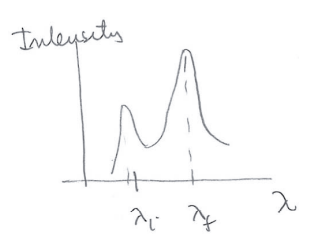
\includegraphics[width=0.5\linewidth]{resources/images/compton-scattering.png}
    \caption{Compton's results at $\theta=90^\circ$.}
    \label{compton-scattering}
\end{figure}

The observed value of $\lambda_f$ is around $0.0731\,\text{nm}$, which aligns quite well with the expected value $\lambda_f=\lambda_i+l_c(m_e)$, where $l_c(m_e)\approx 0.0024\,\text{nm}$. So the second peak makes sense, but how can we interpret the first peak? It represents a process in which the electron remains bound after collision with the photon. Then the entire atom recoils, so the relevant Compton wavelength is that of the atom, which is negligible. Thus, there is no detectable change in the wavelength of the photon.

\subsection{De Broglie's Proposal}
\label{deBroglie_proposal}

By 1924, the wave nature and particle nature of the photon were both certain, but the resolution of how to combine them was unclearly. In that year, Louis de Broglie had the great insight that the photon has a \textbf{particle-wave duality}: both descriptions are required to fully capture its behavior. In fact, he further proposed that \textit{all} matter particles also behave as waves, and that all waves have particle properties. In fact, from Section \ref{schrodinger}, we know that the wave is a \textit{probability wave}. 

Consider a photon. As a particle, it has energy and momentum, and as a wave, it has frequency. This effect is universal; all matter particles have associated \textbf{matter waves}, which represent probability amplitudes. Specifically, for a particle of momentum $p$, we associate with it a plane wave with wavelength $\lambda=\frac{h}{p}$, which is the de Broglie wavelength from Section \ref{compton_wavelength}. This has been experimentally verified by performing the double-slit experiment on increasingly large particles. In fact, we have now performed such experiments on molecules with masses of $10,000$ atomic mass units and de Broglie wavelengths of $1\,pm$. 

\section{Matter Waves \& de Broglie Wavelength}
\label{matter_waves_deBroglie_wavelength}

\subsection{De Broglie Wavelength in Different Frames}
\label{debroglie_in_different_frames}

As we discussed above, de Broglie postulated that a free particle with momentum $p$ can be associated with a plane (matter) wave with wavelength $\lambda=\frac{h}{p}$. Eventually, this wave would become the wavefunction, and the equations describing it would become the Schrödinger equation. In the simplest case, there is only one complex wavefunction $\Psi(\vec{x},\,t)$.

Let's examine the formula $\lambda=\frac{h}{p}$ in more detail. Then $p=\frac{h}{\lambda}=(\frac{h}{2\pi})(\frac{2\pi}{\lambda})=\hbar k$. Consider two non-relativistic observers with rest frames $S$ and $S'$ moving with velocity $+v$ in the $x$-direction relative to $S$. 

Let the particle have mass $m$, velocity $u$ in frame $S$, and velocity $u'$ in frame $S'$. Let its momentum be $p=mu$ in frame $S$ and $p'=mu'$ in frame $S'$. The coordinates are easily related by Galilean transformations: $$x'=x-vt,\;t'=t.$$Then $\frac{dx'}{dt'}=\frac{dx}{dt}-v$. Thus, $u'=u-v$. Similarly, $p'=p-mv$. Therefore, $$\lambda'=\frac{h}{p-mv}\neq\lambda=\frac{h}{p}.$$Thus, the de Broglie wavelength of a particle is dependent on the frame of reference. On the other hand, consider any \textit{measurable} wave. For a general wave, the crucial value is the \textbf{phase} $\phi=kx-\omega t$. The wave itself can be represented as some function of $\phi$. For any point on the wave, all observers will agree on the phase at the point; for this reason, we call the phase a \textbf{Galilean invariant}.

We can rewrite the phase as $$\phi=k(x-\frac{\omega}{k}t)=\frac{2\pi}{\lambda}(x-vt)=\frac{2\pi}{\lambda}x-\frac{2\pi v}{\lambda}t.$$From this expression we see that $k=\frac{2\pi}{\lambda}$ and $\omega=\frac{2\pi v}{\lambda}$. 

\begin{framedtip*}[$k$ and $\omega$]
   Given an expression for the phase of a wave, we can read the wavenumber $k$ and the frequency $\omega$ as the coefficients of $x$ and $t$, respectively. 
\end{framedtip*}

Since phase is a Galilean invariant, we must have $\phi'=\phi$ for all frames $S'$ and $S$. For the same Galilean transformation as above, we have $x=x'+ut'$ and $t=t'$. Thus, $$\frac{2\pi}{\lambda}(x-vt)=\frac{2\pi}{\lambda}(x'+ut'-vt')=\frac{2\pi}{\lambda}x'-\frac{2\pi v}{\lambda}(1-\frac{u}{v})t'.$$Since $k'$ and $\omega'$ are the coefficients of $x'$ and $t'$, respectively, we have $k'=k$ and $\omega'=\omega(1-\frac{u}{v})$. Importantly, since the wavenumber does not change, we must also have $\lambda'=\lambda$. 

We conclude that the wavefunction $\Psi$ is \textit{not} directly measurable, as any directly measurable wave must obey the Galilean invariance above. Additionally, we have found that $\Psi$ is not Galilean invariant: two observers may disagree on the wavefunction at a point in time. That is, for some point measured by two observers as $(x,t)$ and $(x',t')$, we may have $\Psi(x,t)\neq\Psi'(x',t')$. 

\subsection{Frequency of a Matter Wave}
\label{freq_matter_waves}

We have established that a particle with momentum $p$ can be associated with a matter wave of wavenumber $k$ such that $p=\hbar k$. In fact, if the particle has energy $E$, the frequency of the matter wave satisfies $E=\hbar\omega$. These two equations are incredibly important and are together called the \textbf{de Broglie relations}: \begin{align*} \begin{split}
    p&=\hbar k, \\ E&=\hbar\omega.    
\end{split}\tag{de Broglie relations}
\end{align*}

The de Broglie relations on $p$, $k$, $E$, and $\omega$ are fundamental \textit{postulates} of quantum mechanics. That means we cannot derive these relations, but we can test them in specific cases and show that they align with our expectations. Here, we will discuss three pieces of evidence supporting the de Broglie relations. 

\textbf{1. Phase and Group Velocity}

Consider a matter wave with phase $\phi=kx-\omega t$, and assume the de Broglie relations hold. Then the \textbf{phase velocity} $v_p=\frac{\omega}{k}$ of the wave is given by $$v_p=\frac{\omega}{k}=\frac{E}{p}=\frac{\frac{1}{2}mv^2}{mv}=\frac{1}{2}v.$$
Additionally, we define the \textbf{group velocity} $v_g=\frac{d\omega}{dk}$, given by $$v_g=\frac{d\omega}{dk}\bigg|_k=\frac{dE}{dp}=\frac{d}{dp}(\frac{p^2}{2m})=\frac{p}{m}=v.$$
Notice that the phase velocity, which is the speed of a \textit{single wave crest} through the medium, is half the velocity of the particle. When the phase velocity is constant, as in a sine wave, we have a \textbf{plane wave}. Plane waves cannot carry any information, so a particle cannot be represented by a plane wave. Instead, it must be represented by a \textbf{wavepacket}, which we will discuss soon. For this reason, the phase velocity is not very meaningful.

On the other hand, the group velocity, which represents the speed of the \textit{wavepacket}, perfectly equals the speed of the particle. In fact, $v_g=v$ even for relativistic particles. Thus, the de Broglie relations cause matter waves to move with the same speed as particles, which is evidence that they are true.

\textbf{2. Four-Vectors}

If you happen to have studied special relativity, you will recall that the four-momentum is defined as $\vec{P}=(\frac{E}{c},\,\vec{p})$ (if not, don't worry --- this is the only relativity in this course!). Similarly, for a wave whose phase is relativistically invariant, $(\frac{\omega}{c},\,k)$  is also a four-vector. Then both de Broglie relations follow from equating two four-vectors: $$(\frac{E}{c},\,\vec{p})=\hbar(\frac{\omega}{c},\,\vec{k}).$$ This supports the de Broglie relations because they would then be true in all Lorentz frames. In other words, this shows that the de Broglie relations are consistent relativistically.

\textbf{3. Photons}

For photons, the de Broglie relations agree with Einstein's energy quanta: $E_\gamma=h\nu=\hbar\omega.$ In the footnote on page 16, we saw that photons also have momentum $p_\gamma=\frac{\hbar}{\lambda}=\hbar k$. We can therefore think of the de Broglie relations as simply extending Einstein's findings for photons to matter particles.

\section{Wavepackets}
\label{wavepackets}
\subsection{Stationary Phase Approximation}
\label{stationary_phase_approximation}

Suppose we have some function of frequency in terms of wavenumber $\omega(k)$. As defined in Section \ref{freq_matter_waves}, the group velocity is $v_g=\frac{d\omega}{dk}$ and represents the velocity of a ``packet'' constructed by superimposing waves. Figure \ref{wavepacket} shows a screenshot of a wavepacket, its sinusoidal wave components, and the component amplitudes.\footnote{This screenshot is from the PhET \href{https://phet.colorado.edu/en/simulations/fourier-making-waves} {\textit{Fourier: Making Waves \emph{simulation}}}. The PhET interactive simulations are excellent resources created by the University of Colorado.}

\begin{figure}[H]
    \centering
    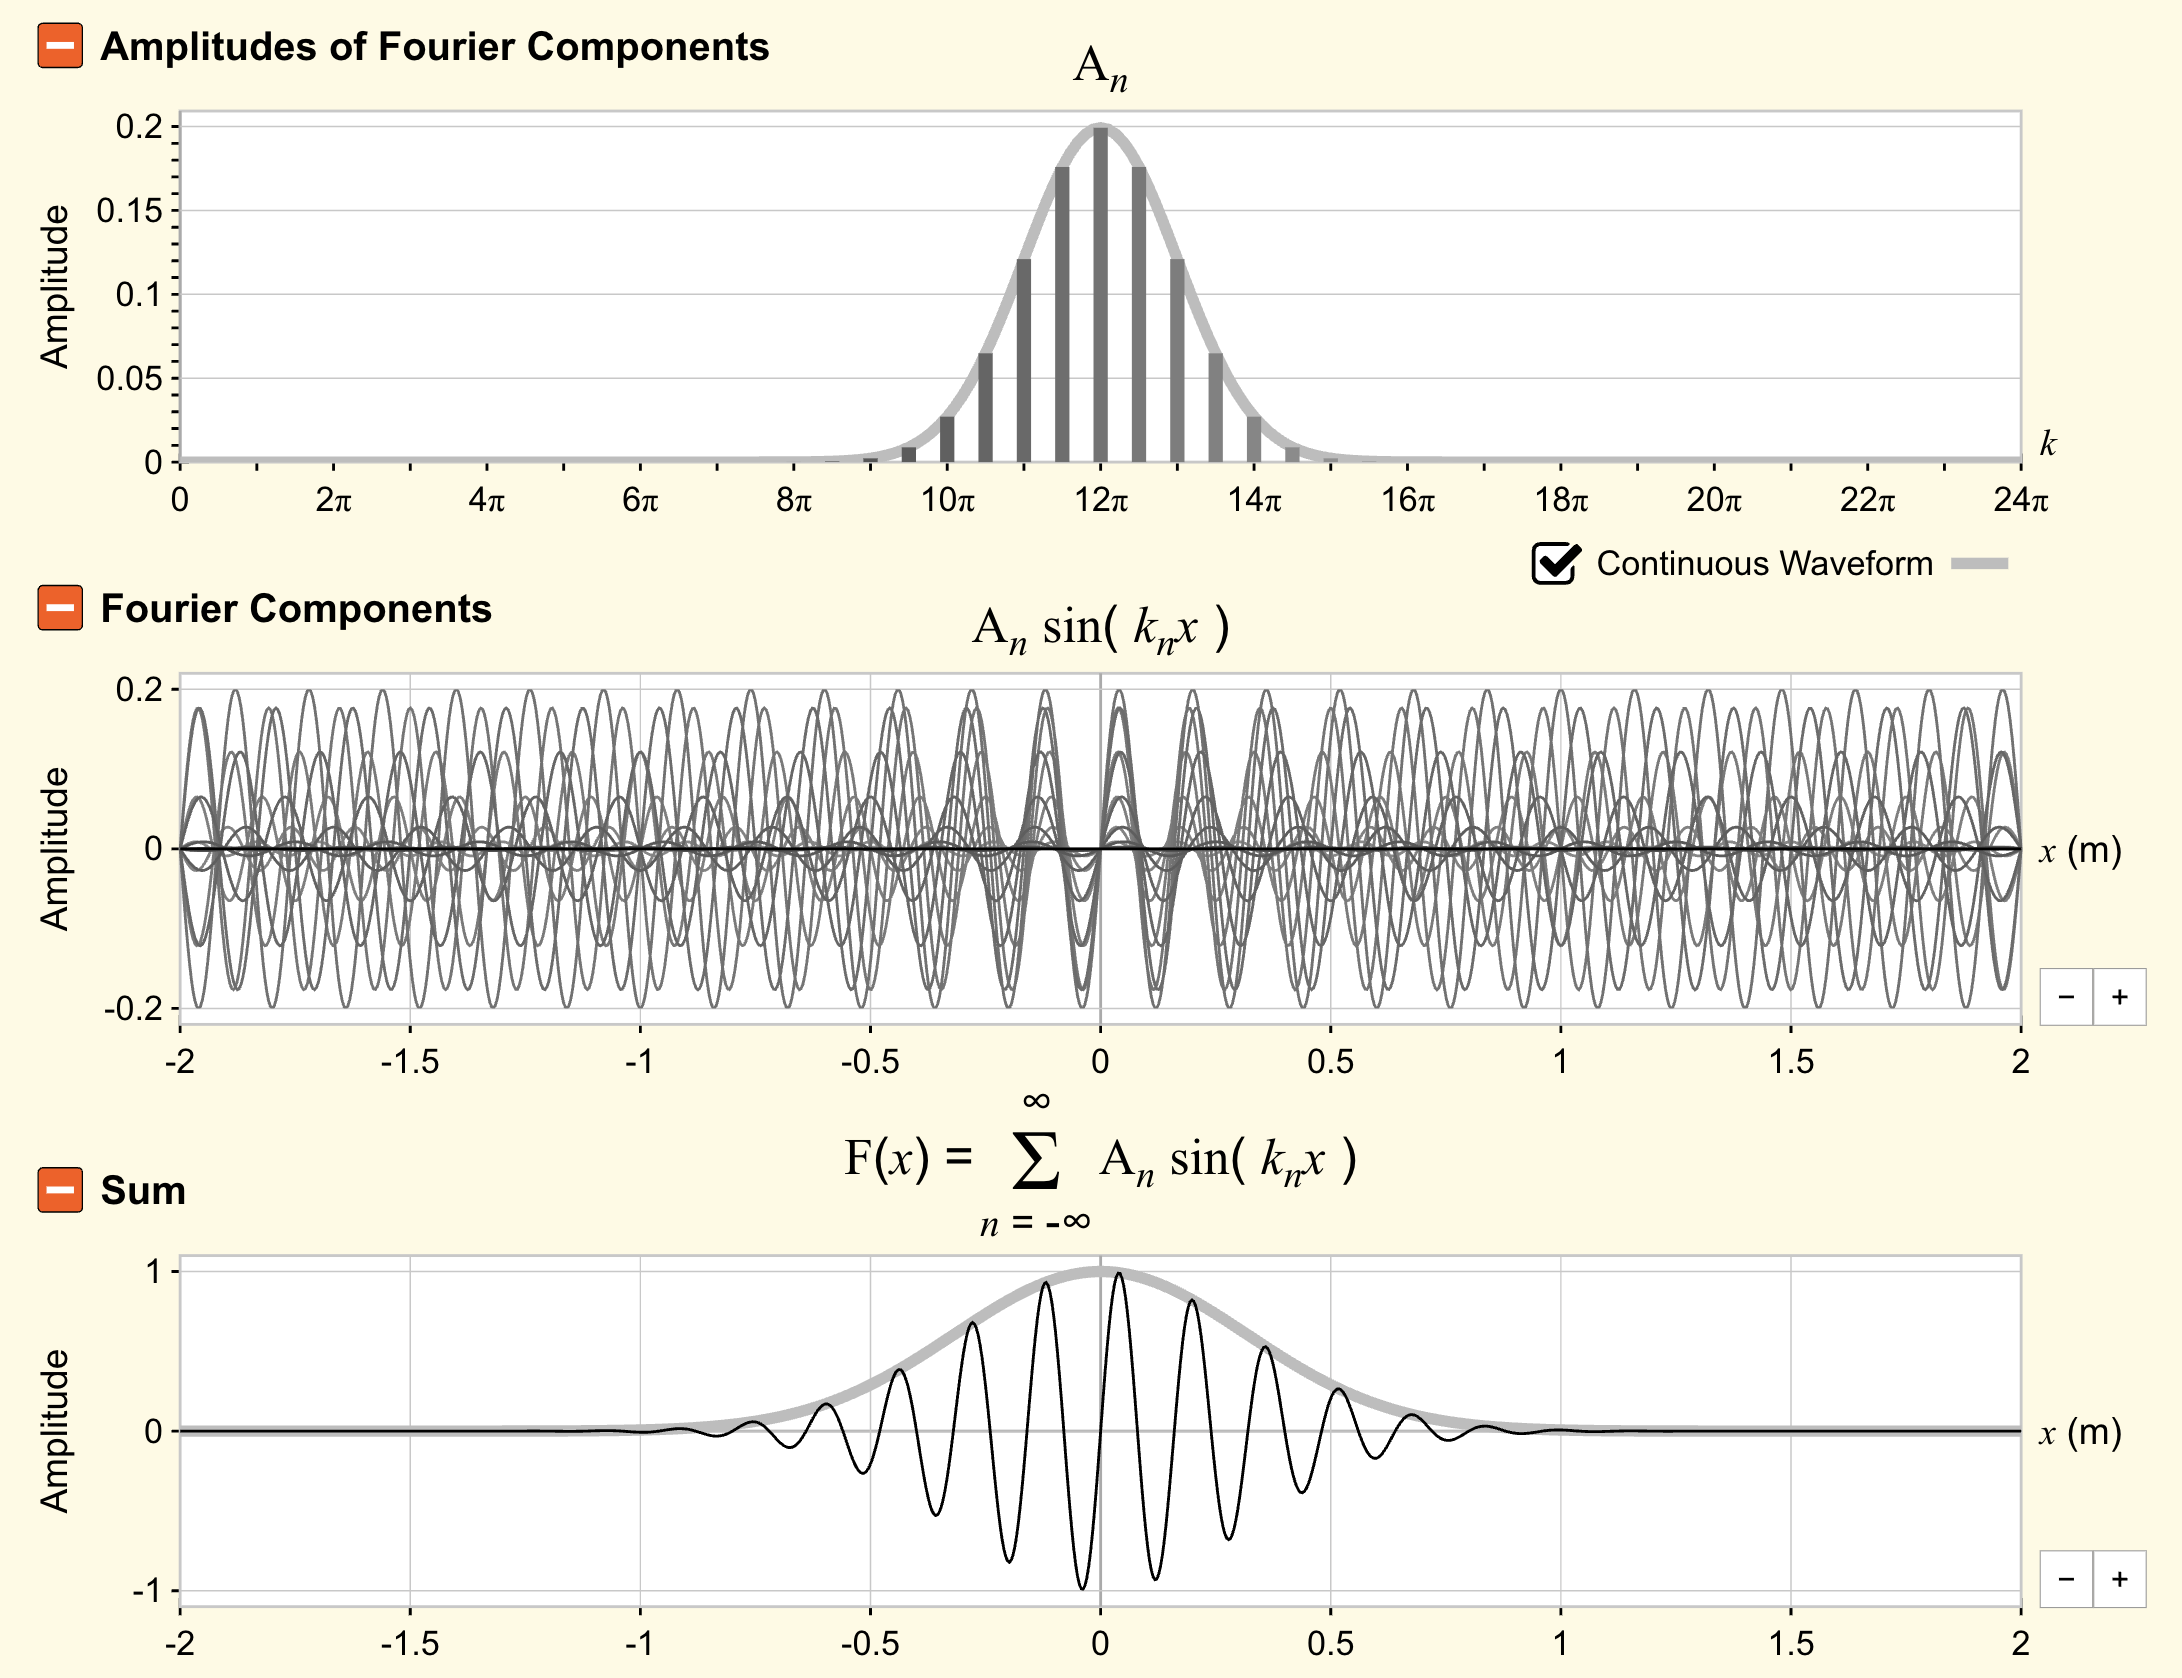
\includegraphics[width=0.8\linewidth]{resources/images/wavepacket.png}
    \caption{Top to bottom: a graph of the amplitudes of the component waves ($\Phi(k)$ below), a graph of the component waves ($\Phi(k)e^{i\phi(k)}$), and a graph of the wavepacket ($\int dk\,\Phi(k)e^{i\phi(k)}$).}
    \label{wavepacket}
\end{figure}
Consider the general wavefunction representing the superposition of infinitely many waves of phase $\phi(k)=kx-\omega(k)t$ and amplitude $\Phi(k)$:$$\Psi(x,\,t)=\int dk\;\Phi(k)e^{i\phi(k)}.$$We also assume that $\Phi(k)$ is both real and 0 almost everywhere, except for a narrow peak around a value $k_0$. In Figure \ref{wavepacket}, $k_0=12\pi$. We would like to see how the wavefunction behaves over time. There is a quick way of seeing this, called the \textbf{principle of stationary phase}, or the stationary phase approximation. 

\begin{framedthm}[Principle of stationary phase]\label{principle_stationary_phase}
    The integral of a function $f(x)$ multiplied by some rapidly oscillating value like $\sin(\phi(x))$ will be approximately 0 except in places with small oscillating frequency. 
\end{framedthm}

Here, the function is $\Phi(k)$ and the oscillating value is $e^{i\phi(k)}$. Since the integral only has a chance to be nonzero at $k\approx k_0$ where $\Phi(k)\neq 0$, the phase must be stationary with respect to $k$ at this point. And since we assumed $\Phi(k)$ to be real, the phase is only contributed by $\phi(k)=kx-\omega(k)t$. Thus, we must have $$\frac{d\phi(k)}{dk}\bigg|_{k_0}=x-\frac{d\omega(k)}{dk}\bigg|_{k_0}t=0.$$Then we need $\frac{d\omega(k)}{dt}=\frac{x}{t}$, which confirms that the group velocity $v_g=\frac{d\omega(k)}{dt}$ is indeed the speed of the wavepacket.

\subsection{Group Velocity}\label{group_velocity}

We can also show this result without approximating. We rewrite the wavefunction $$\Psi(x,\,t)=\int dk\;\Phi(k)e^{i(kx-\omega(k) t)}.$$At time $t=0$, we have $$\Psi(x,\,0)=\int dk\;\Phi(k)e^{ikx}.$$Since the integral is only nonzero for $k\approx k_0$, we linearly approximate $\omega(k)$ as $$\omega(k)= \omega(k_0)+ (k-k_0)\frac{d\omega(k)}{dt}\bigg|_{k_0}+O((k-k_0)^2).$$Substituting back into the integral, $$\Psi(x,\,t)=\int dk\;\Phi(k)\,e^{ikx}\,e^{-i\omega(k_0) t}\,e^{-ik\frac{d\omega}{dk}|{k_0}t}\,e^{ik_0\frac{d\omega}{dk}|_{k_0}t}.$$ Our integral is now looking pretty bad. However, note that the second and fourth exponential factors are independent of $k$! We can take these out of the integral to get $$\Psi(x,\,t)=e^{-i\omega(k_0) t}\,e^{ik_0\frac{d\omega}{dk}|_{k_0}t}\int dk\;\Phi(k)\,e^{ik(x-\frac{d\omega}{dk}|{k_0}t)}.$$The integral can now be written in terms of the wavefunction at time 0. Taking the magnitude of both sides to remove the annoying exponential phases outside the integral, we see that $$|\Psi(x,\,t)|=|\Psi(x-\frac{d\omega}{dk}\bigg|_{k_0}t,\,0)|.$$Just as in Section \ref{stationary_phase_approximation}, we see that the wavepacket moves with speed given by the group velocity $v_g= \frac{d\omega}{dk}|_{k_0}$.
